\documentclass[tikz,border=6pt]{standalone}
% Shared visual language for the original benchmark atlas.
\usepackage[T1]{fontenc}
\usepackage{lmodern}
\usepackage{amsmath,amssymb}
\usetikzlibrary{arrows.meta,calc,positioning,shapes.geometric,patterns,decorations.pathmorphing,backgrounds,fit}
\definecolor{ink}{HTML}{173948}
\definecolor{flow}{HTML}{167D9A}
\definecolor{control}{HTML}{A65217}
\definecolor{measure}{HTML}{70518A}
\definecolor{pale}{HTML}{EAF2F5}
\definecolor{muted}{HTML}{526571}
\definecolor{utility}{HTML}{2E8665}
\tikzset{
  every node/.style={font=\sffamily\small,text=ink},
  equipment/.style={draw=ink,line width=1pt,fill=pale,rounded corners=2pt},
  process/.style={draw=flow,line width=1.2pt,-{Latex[length=2.5mm]}},
  signal/.style={draw=control,line width=.8pt,dashed,-{Latex[length=2mm]}},
  util/.style={draw=utility,line width=1pt,-{Latex[length=2.2mm]}},
  dimension/.style={draw=muted,line width=.6pt,{Latex[length=1.7mm]}-{Latex[length=1.7mm]}},
  labelbox/.style={fill=white,inner sep=2pt,font=\sffamily\footnotesize,align=center},
  annotation/.style={font=\sffamily\footnotesize,text=muted,align=left},
  panel/.style={draw=ink!20,fill=ink!2,rounded corners=3pt,inner sep=6pt},
  instrument/.style={circle,draw=measure,fill=white,line width=.8pt,minimum size=8mm,inner sep=1pt,font=\sffamily\scriptsize,align=center},
  port/.style={circle,fill=flow,inner sep=1.6pt},
  box/.style={equipment,minimum width=3cm,minimum height=1cm,align=center},
}
\newcommand{\atlasheader}[3]{%
  \node[anchor=north west,font=\sffamily\bfseries\LARGE] at (0,0) {#1};%
  \node[anchor=north west,font=\sffamily\small,text=muted] at (0,-.75) {Paper section #2: \textit{#3}};%
  \draw[ink!25,line width=.7pt] (0,-1.25)--(26,-1.25);%
}
\newcommand{\atlasfooter}[1]{%
  \draw[ink!25,line width=.5pt] (0,-15.8)--(26,-15.8);%
  \node[anchor=north west,annotation,text width=25.8cm] at (0,-16) {#1\\Original explanatory drawing. Source: Kroll \& Schulte (2014), DOI: 10.1016/j.asoc.2014.08.034. Model variants are identified in the accompanying case sheet.};%
}

% Primary diagram reference: TikZ.net (user preference, see repository AGENTS.md).
% https://tikz.net/fluid_dynamics_laminar/ -- explicit styles, rounded paths.
% https://tikz.net/mechanics/ -- named coordinates and separately placed labels.
% https://tikz.net/fluid_dynamics_barometer/ -- pipe arcs and label anchors.
\newcommand{\diagramlabel}{\sffamily\fontsize{8}{9.5}\selectfont}
\newcommand{\equipmentfont}{\sffamily\bfseries\fontsize{9}{10.5}\selectfont}
% Natural industrial finishes: painted machinery, reflective steel and clear cutaways.
% Blue machinery is inspired by real industrial motor/compressor finishes; this is
% not a specified vendor, alloy, piping standard or measured A--H chemical colour.
% Finish references: WEG electric-motor colour catalog (W22 Premium, RAL 5009),
% https://static.weg.net/medias/downloadcenter/h26/h37/WEG-cores-dos-motores-eletricos-weg-50029349-catalogo-portugues-br.pdf
% https://www.copeland.com/pt-br/products-solutions/compression-technologies-systems/industrial-reciprocating-compressors
\definecolor{ink}{HTML}{263B43}
\definecolor{flow}{HTML}{66736F}
\definecolor{utility}{HTML}{2F7B76}
\definecolor{steamline}{HTML}{94816B}
\definecolor{liquid}{HTML}{C6DED7}
\definecolor{liquidlight}{HTML}{F3FAF3}
\definecolor{level}{HTML}{79A29B}
\definecolor{pale}{HTML}{F7F6F0}
\definecolor{muted}{HTML}{576C70}
\definecolor{steel}{HTML}{CBD2D3}
\definecolor{steelshadow}{HTML}{879FA8}
\definecolor{steelwarm}{HTML}{C7BCAB}
\definecolor{steelhighlight}{HTML}{F7F4E8}
\definecolor{steeledge}{HTML}{526A73}
\definecolor{machineblue}{HTML}{176889}
\definecolor{machineshadow}{HTML}{123F56}
\definecolor{machinehighlight}{HTML}{6FA6BA}
\definecolor{actuator}{HTML}{39738B}
\tikzset{
  equipment/.style={draw=steeledge,line width=1.05pt,fill=pale,rounded corners=2pt},
  metal/.style={shade,left color=steelshadow,right color=steelwarm,middle color=steelhighlight},
  metalcross/.style={shade,top color=steelwarm,bottom color=steelshadow,middle color=steelhighlight},
  machinepaint/.style={shade,left color=machineshadow,right color=machineblue,middle color=machinehighlight},
  shell/.style={draw=steeledge,line width=1.05pt},
  cutaway/.style={draw=steelshadow!65,line width=.45pt,fill=pale,fill opacity=.66,draw opacity=1},
  pipe/.style={draw=flow,line width=1.25pt,line cap=round,line join=round,rounded corners=2.5pt},
  process/.style={pipe,-{Triangle[length=2.6mm,width=1.8mm,fill=ink,color=ink]}},
  utilpipe/.style={draw=utility,line width=1.05pt,line cap=round,line join=round,rounded corners=2.5pt},
  util/.style={utilpipe,-{Triangle[length=2.4mm,width=1.7mm,fill=ink,color=ink]}},
  steam/.style={util,draw=steamline},
  tag/.style={circle,draw=flow,line width=.6pt,fill=white,inner sep=1.7pt,font=\diagramlabel},
  smallnote/.style={annotation,font=\diagramlabel},
  labelbox/.style={fill=white,inner sep=2pt,font=\diagramlabel,align=center},
  equipmenttitle/.style={font=\equipmentfont,inner sep=1.5pt,align=center},
  liquidlevel/.style={draw=level,line width=.8pt},
}
% One shared centreline for the pipe, valve body, stem and closed actuator.
\newcommand{\valve}[3]{%
  \begin{scope}[shift={(#1,#2)}]
    \path[draw=ink,fill=steelhighlight,line width=.75pt]
      (-.23,-.18)--(0,0)--(-.23,.18)--cycle
      (.23,-.18)--(0,0)--(.23,.18)--cycle;
    \draw[ink,line width=.7pt](0,0)--(0,.44);
    \path[draw=actuator,fill=actuator!12!white,line width=.7pt]
      (-.16,.44)arc(180:0:.16)--cycle;
    \node[font=\diagramlabel,anchor=south,inner sep=1.5pt]at(0,.72){#3};
  \end{scope}%
}
\begin{document}
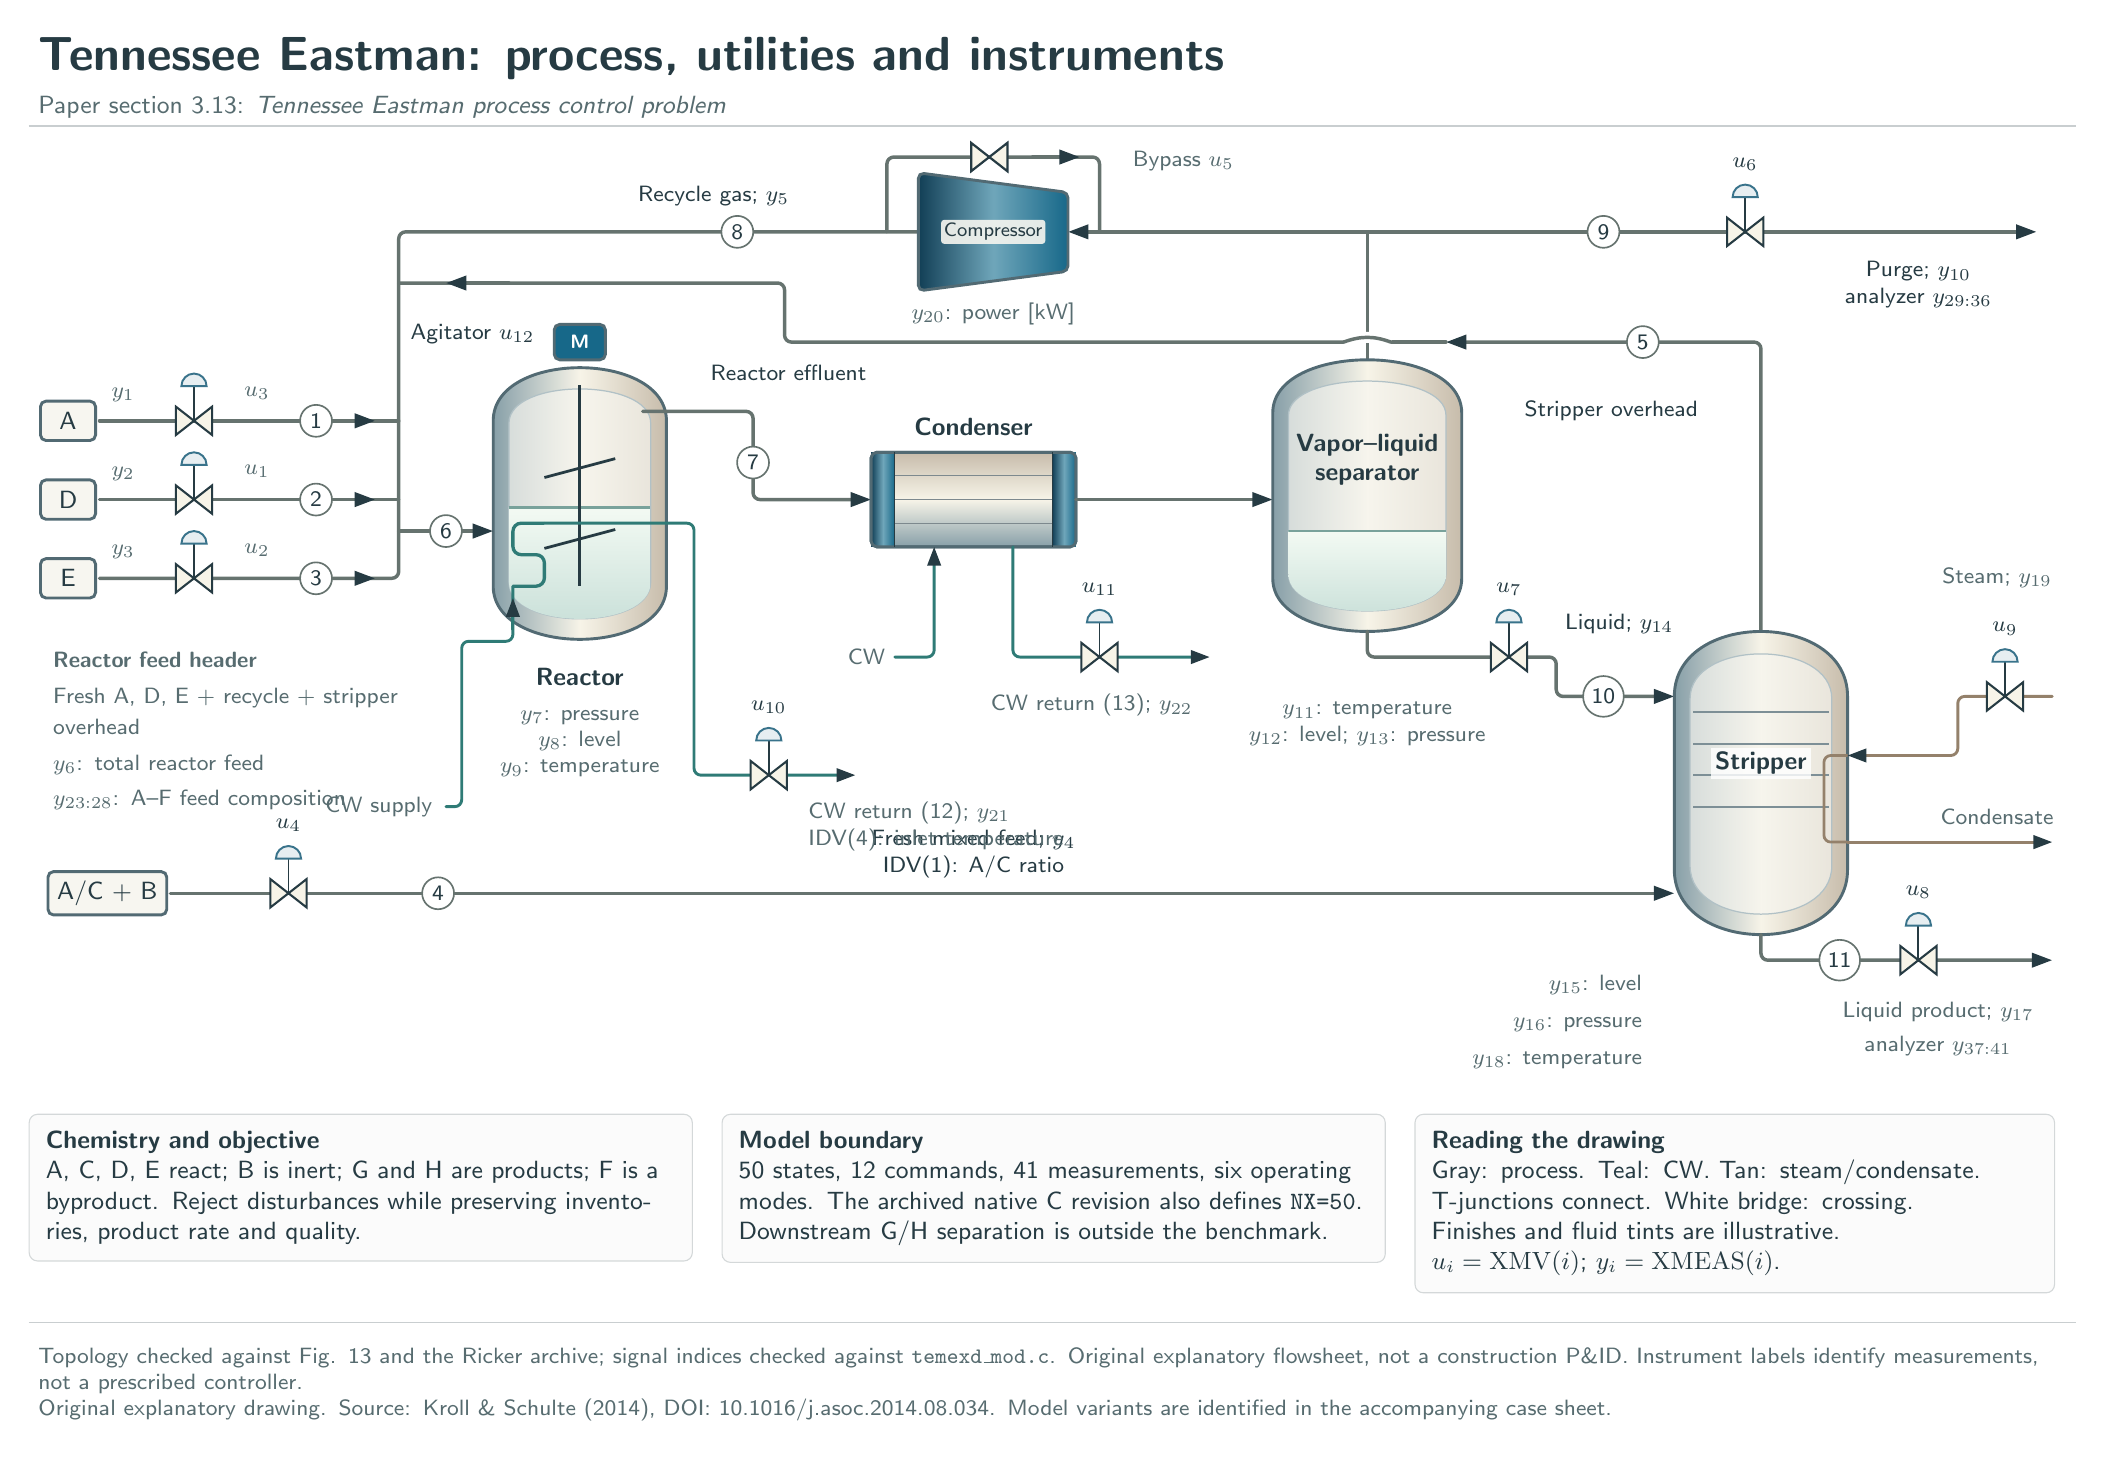
\begin{tikzpicture}[x=1cm,y=1cm]
\atlasheader{Tennessee Eastman: process, utilities and instruments}{3.13}{Tennessee Eastman process control problem}
% Exact midpoints of the curved vessel heads; valve coordinates share pipe y.
\coordinate (separator-top) at (17,-4.225);
\coordinate (separator-bottom) at (17,-7.675);
\coordinate (separator-outlet) at (17,-8.0);
\coordinate (stripper-bottom) at (22,-11.525);
% Recycle first, with a compressor bypass rather than a fictitious feed valve.
% Split true tees into straight segments: rounded elbows must not open a junction.
\draw[pipe](separator-top)--(17,-2.6);
\draw[process](17,-2.6)--(13.2,-2.6);
\draw[pipe](11.3,-2.6)--(4.7,-2.6)--(4.7,-6.4);
% TikZ.net node padding: keep the nameplate inset from the compressor shell.
\path[equipment,machinepaint](13.2,-2.1)--(13.2,-3.1)--(11.3,-3.35)--(11.3,-1.85)--cycle;
\node[smallnote,font=\sffamily\fontsize{7.5}{9}\selectfont,text=ink,fill=pale,fill opacity=.9,text opacity=1,rounded corners=1pt,inner xsep=1pt,inner ysep=1.2pt,align=center]at(12.25,-2.6){Compressor};
% A dedicated label band separates power measurement, casing and return pipe.
\node[smallnote,align=center,inner sep=2pt]at(12.25,-3.64){$y_{20}$: power [kW]};
\draw[pipe](10.9,-2.6)--(10.9,-1.65)--(13.6,-1.65)--(13.6,-2.6);
\draw[process](12.75,-1.65)--(13.35,-1.65);
\path[draw=ink,fill=steelhighlight,line width=.8pt](11.97,-1.83)--(12.43,-1.47)--(12.43,-1.83)--(11.97,-1.47)--cycle;
\node[smallnote,anchor=west]at(13.9,-1.7){Bypass $u_5$};
\node[tag]at(9,-2.6){8};\node[labelbox,anchor=south]at(8.7,-2.35){Recycle gas; $y_5$};
\draw[process](17,-2.6)--(25.5,-2.6);
\valve{21.8}{-2.6}{$u_6$}
\node[tag]at(20,-2.6){9};\node[labelbox,anchor=north]at(24,-2.9){Purge; $y_{10}$\\analyzer $y_{29:36}$};
% Major vessels and internal details.
\def\reactoroutline{(5.9,-5.0)..controls(5.9,-4.1)and(8.1,-4.1)..(8.1,-5.0)--(8.1,-7.1)..controls(8.1,-8.0)and(5.9,-8.0)..(5.9,-7.1)--cycle}
\def\reactorcutaway{(6.10,-5.03)..controls(6.10,-4.45)and(7.90,-4.45)..(7.90,-5.03)--(7.90,-7.05)..controls(7.90,-7.67)and(6.10,-7.67)..(6.10,-7.05)--cycle}
\path[metal]\reactoroutline;
\path[cutaway]\reactorcutaway;
\begin{scope}
  \clip\reactorcutaway;
  \shade[top color=liquidlight,bottom color=liquid](6.10,-6.1)rectangle(7.90,-7.7);
  \draw[liquidlevel](6.10,-6.1)--(7.90,-6.1);
\end{scope}
\draw[shell]\reactoroutline;
\draw[ink,line width=1.2pt](7,-4.55)--(7,-7.1);
\foreach \yy in {-5.6,-6.5}{\draw[ink,line width=1pt](6.55,\yy-.12)--(7.45,\yy+.12);}
\node[equipment,fill=machineblue,text=white,minimum width=.65cm,minimum height=.45cm]at(7,-4.0){\scriptsize\bfseries M};
\node[labelbox,anchor=east]at(6.5,-3.9){Agitator $u_{12}$};
\draw[utility,line width=1.2pt,rounded corners=3pt](6.55,-6.3)--(6.15,-6.3)--(6.15,-6.7)--(6.55,-6.7)--(6.55,-7.1)--(6.15,-7.1);
\node[equipmenttitle](reactor-title)at(7,-8.25){Reactor};
% TikZ.net mechanics example: anchor annotations independently of nearby paths.
% One measurement per line keeps an open margin to both cooling-water pipes.
\node[smallnote,align=center,anchor=north,inner sep=1.5pt]
  at([yshift=-2mm]reactor-title.south)
  {$y_7$: pressure\\$y_8$: level\\$y_9$: temperature};
% Allow a distinct corridor between the overhead return and reactor effluent.
\draw[process](7.8,-4.88)--(9.2,-4.88)--(9.2,-6.0)--(10.7,-6.0);
\node[tag]at(9.2,-5.53){7};
\node[labelbox,anchor=south,inner sep=1.4pt]at(9.65,-4.55){Reactor effluent};
\draw[equipment,metalcross](10.7,-5.4)rectangle(13.3,-6.6);
\path[machinepaint](10.7,-5.4)rectangle(11.0,-6.6);
\path[machinepaint](13.0,-5.4)rectangle(13.3,-6.6);
\draw[shell,rounded corners=2pt](10.7,-5.4)rectangle(13.3,-6.6);
\draw[ink](11.0,-5.4)--(11.0,-6.6)(13.0,-5.4)--(13.0,-6.6);
\foreach \yy in {-5.7,-6.0,-6.3}{\draw[ink!60](11,\yy)--(13,\yy);}
\node[equipmenttitle,anchor=south]at(12,-5.25){Condenser};
\draw[process](13.3,-6)--(15.8,-6);
\def\separatoroutline{(15.8,-4.9)..controls(15.8,-4.0)and(18.2,-4.0)..(18.2,-4.9)--(18.2,-7.0)..controls(18.2,-7.9)and(15.8,-7.9)..(15.8,-7.0)--cycle}
\def\separatorcutaway{(16.00,-4.93)..controls(16.00,-4.35)and(18.00,-4.35)..(18.00,-4.93)--(18.00,-6.95)..controls(18.00,-7.57)and(16.00,-7.57)..(16.00,-6.95)--cycle}
\path[metal]\separatoroutline;
\path[cutaway]\separatorcutaway;
\begin{scope}
  \clip\separatorcutaway;
  \shade[top color=liquidlight,bottom color=liquid](16.00,-6.4)rectangle(18.00,-7.6);
  \draw[liquidlevel](16.00,-6.4)--(18.00,-6.4);
\end{scope}
\draw[shell]\separatoroutline;
\node[equipmenttitle]at(17,-5.5){Vapor--liquid\\separator};
\node[smallnote,align=center]at(17,-8.85){$y_{11}$: temperature\\$y_{12}$: level; $y_{13}$: pressure};
% Stripper overhead returns to reactor header. White bridge = crossing, no junction.
\draw[process](22,-7.7)--(22,-4.0)--(18,-4.0);
\draw[pipe](18,-4)--(17.3,-4);
\draw[pipe,preaction={draw=white,line width=4pt}](17.3,-4)to[out=160,in=20](16.7,-4);
\draw[pipe](16.7,-4)--(9.6,-4)--(9.6,-3.25)--(4.7,-3.25);
\draw[process](6.1,-3.25)--(5.3,-3.25);
\node[tag]at(20.5,-4){5};
% Keep the overhead caption below (not against) the horizontal return line.
\node[labelbox,anchor=north,inner sep=2pt]at(20.1,-4.67){Stripper overhead};
% Fresh feeds A,D,E join recycle and stripper overhead at the reactor header.
\foreach \yy/\sp/\st/\uv/\ym in {-5.0/A/1/3/1,-6.0/D/2/1/2,-7.0/E/3/2/3}{
  \node[equipment,minimum width=.7cm,minimum height=.5cm]at(.5,\yy){\sp};
  \ifnum\st=3
    \draw[pipe](.9,\yy)--(4.7,\yy)--(4.7,-6.4);
  \else
    \draw[pipe](.9,\yy)--(4.7,\yy);
  \fi
  % Direction markers sit on straight runs, clear of the unmarked tee joints.
  \draw[process](4.0,\yy)--(4.4,\yy);
  \valve{2.1}{\yy}{}
  \node[smallnote,anchor=south]at(2.9,\yy+.15){$u_{\uv}$};
  \node[tag]at(3.65,\yy){\st};
  \node[smallnote,anchor=south]at(1.2,\yy+.12){$y_{\ym}$};
}
\draw[process](4.7,-6.4)--(5.9,-6.4);
\node[tag]at(5.3,-6.4){6};
% Increase line leading and separate heading/composition from the dense feed pipes.
% TikZ.net mechanics: keep a separate, padded and explicitly anchored label node.
\node[smallnote,anchor=north west,align=left,text width=4.7cm,
      font=\sffamily\fontsize{8}{11.2}\selectfont,
      inner xsep=3pt,inner ysep=3pt]
  at(.2,-7.83){\textbf{Reactor feed header}\\[1.5pt]
    Fresh A, D, E + recycle + stripper overhead\\[2pt]
    $y_6$: total reactor feed\\[1.5pt]
    $y_{23:28}$: A--F feed composition};
% Separator liquid and stripper with a heating circuit.
\draw[process](separator-bottom)--(separator-outlet)--(19.4,-8.0)--(19.4,-8.5)--(20.9,-8.5);
\valve{18.8}{-8.0}{$u_7$}
\node[tag]at(20,-8.5){10};\node[labelbox,anchor=south]at(20.2,-7.78){Liquid; $y_{14}$};
\def\stripperoutline{(20.9,-8.5)..controls(20.9,-7.4)and(23.1,-7.4)..(23.1,-8.5)--(23.1,-10.7)..controls(23.1,-11.8)and(20.9,-11.8)..(20.9,-10.7)--cycle}
\def\strippercutaway{(21.10,-8.53)..controls(21.10,-7.77)and(22.90,-7.77)..(22.90,-8.53)--(22.90,-10.65)..controls(22.90,-11.47)and(21.10,-11.47)..(21.10,-10.65)--cycle}
\path[metal]\stripperoutline;
\path[cutaway]\strippercutaway;
\draw[shell]\stripperoutline;
\foreach \yy in {-8.7,-9.1,-9.5,-9.9}{\draw[steeledge!75,line width=.65pt](21.14,\yy)--(22.86,\yy);}
\node[labelbox,equipmenttitle,fill=white,fill opacity=.82,text opacity=1]at(22,-9.35){Stripper};
% Keep the stripper measurements in their own left-aligned spatial zone.
\node[smallnote,anchor=north east,align=right,
      font=\sffamily\fontsize{8}{11.8}\selectfont,inner sep=1.5pt]
  at(20.55,-11.98){$y_{15}$: level\\[1.5pt]
    $y_{16}$: pressure\\[1.5pt]
    $y_{18}$: temperature};
\node[equipment,minimum width=1.5cm,minimum height=.55cm]at(1,-11.0){A/C + B};
\draw[process](1.8,-11)--(20.9,-11);
\valve{3.3}{-11}{$u_4$}
\node[tag]at(5.2,-11){4};\node[labelbox,anchor=south]at(12.0,-10.88){Fresh mixed feed; $y_4$\\IDV(1): A/C ratio};
\draw[process](stripper-bottom)--(22,-11.85)--(25.7,-11.85);
\valve{24}{-11.85}{$u_8$}
\node[tag]at(23,-11.85){11};
% Product quality is centered under the outlet, not in the measurement column.
\node[smallnote,anchor=north,align=center,text width=3.0cm,
      font=\sffamily\fontsize{8}{11.5}\selectfont,inner sep=1.5pt]
  at(24.25,-12.32){Liquid product; $y_{17}$\\[1pt]
    analyzer $y_{37:41}$};
% Utilities: separate colored lines and explicit inlet/outlet directions.
% Place the inlet arrow on a straight run, clear of the coil's final elbow.
% Separate the utility caption from the feed header above and valve tag u_4.
\draw[utilpipe](5.3,-9.9)--(5.5,-9.9)--(5.5,-7.8)--(6.15,-7.8)--(6.15,-7.1);
\draw[util](6.15,-7.65)--(6.15,-7.25);
\node[smallnote,anchor=east]at(5.25,-9.9){CW supply};
\draw[util](6.55,-6.3)--(8.45,-6.3)--(8.45,-9.5)--(10.5,-9.5);
\valve{9.4}{-9.5}{$u_{10}$}
\node[smallnote,anchor=north west,align=left]at(9.78,-9.72){CW return (12); $y_{21}$\\IDV(4): inlet temperature};
\draw[util](11,-8.0)--(11.5,-8.0)--(11.5,-6.6);
\node[smallnote,anchor=east]at(11,-8){CW};
\draw[util](12.5,-6.6)--(12.5,-8)--(15,-8);
\valve{13.6}{-8}{$u_{11}$}
\node[smallnote,anchor=north]at(13.5,-8.35){CW return (13); $y_{22}$};
\draw[steam](25.7,-8.5)--(24.5,-8.5)--(24.5,-9.25)--(23.1,-9.25);
\valve{25.1}{-8.5}{$u_9$}
\node[smallnote,anchor=south]at(25,-7.25){Steam; $y_{19}$};
\draw[steamline,line width=1pt,rounded corners=2.5pt](23.1,-9.25)--(22.8,-9.25)--(22.8,-10.35)--(23.1,-10.35);
\draw[steam](23.1,-10.35)--(24.5,-10.35)--(25.7,-10.35);
\node[smallnote,anchor=south]at(25,-10.25){Condensate};
% Readable explanatory panels, not a claim of industrial P&ID completeness.
% TikZ.net spacing reference: reserve a clear band below the process annotations.
% Shift the panel row and footer together so their mutual spacing stays fixed.
\begin{scope}[yshift=-6.5mm]
\node[panel,anchor=north west,text width=8cm,minimum height=1.7cm,align=left]at(0,-13.15){\textbf{Chemistry and objective}\\A, C, D, E react; B is inert; G and H are products; F is a byproduct. Reject disturbances while preserving inventories, product rate and quality.};
\node[panel,anchor=north west,text width=8cm,minimum height=1.7cm,align=left]at(8.8,-13.15){\textbf{Model boundary}\\50 states, 12 commands, 41 measurements, six operating modes. The archived native C revision also defines \texttt{NX=50}. Downstream G/H separation is outside the benchmark.};
\node[panel,anchor=north west,text width=7.7cm,minimum height=1.7cm,align=left]at(17.6,-13.15){\textbf{Reading the drawing}\\Gray: process. Teal: CW. Tan: steam/condensate.\\T-junctions connect. White bridge: crossing.\\Finishes and fluid tints are illustrative.\\$u_i=\mathrm{XMV}(i)$; $y_i=\mathrm{XMEAS}(i)$.};
\atlasfooter{Topology checked against Fig. 13 and the Ricker archive; signal indices checked against \texttt{temexd\_mod.c}. Original explanatory flowsheet, not a construction P\&ID. Instrument labels identify measurements, not a prescribed controller.}
\end{scope}
\end{tikzpicture}
\end{document}
